
\section{Ход выполнения работы}

\subsection{Описание конфигурации кластера}

Работа выполнена в среде VirtualBox на трёх виртуальных машинах
под управлением AlmaLinux 9: двух серверах хранения \texttt{node1}, \texttt{node2}
и клиенте \texttt{mgmt}. Конфигурация узлов приведена в таблице~\ref{tab:nodes}.

\begin{table}[h]
    \centering
    \caption{Узлы кластера}
    \label{tab:nodes}
    \begin{tabular}{|l|l|l|l|}
        \hline
        Имя хоста & IP-адрес & Роль в кластере & Роль в GlusterFS \\
        \hline
        \texttt{node1} & 10.0.2.11 & сервер хранения & сервер (glusterd), брики \\
        \hline
        \texttt{node2} & 10.0.2.12 & сервер хранения & сервер (glusterd), брики \\
        \hline
        \texttt{mgmt} & 10.0.2.10 & клиент & клиент (glusterfs-fuse) \\
        \hline
    \end{tabular}
\end{table}

Каждая машина имеет диск объемом 20 ГБ с файловой системой XFS.
На серверах \texttt{node1} и \texttt{node2} дополнительно установлены
виртуальные диски объемом 4 ГБ для размещения бриков тома со снимками.
Используемая версия GlusterFS --- 11.2.

Основные понятия GlusterFS:
\begin{itemize}
    \item \texttt{brick} --- каталог на сервере, в котором физически
    хранятся данные тома;
    \item доверенный пул (trusted pool) --- группа серверов, объединенных
    в кластер GlusterFS;
    \item том (volume) --- логическое хранилище, собранное из нескольких
    бриков;
    \item \texttt{glusterd} --- служба управления GlusterFS;
    \item \texttt{glusterfs-fuse} --- клиент, позволяющий смонтировать том
    как обычный каталог.
\end{itemize}

\subsection{Подготовка узлов}

Перед установкой на всех узлах были проверены версия ОС, сетевые
адреса и связность между машинами (листинг~\ref{lst:check}).

\begin{lstlisting}[caption={Проверка узлов (node1, node2, mgmt)}, label={lst:check}]
cat /etc/os-release
hostname -I
ping -c 2 10.0.2.11
ping -c 2 10.0.2.12
ping -c 2 10.0.2.10
\end{lstlisting}

Узлы уже были доступны по IP-адресам, а имена хостов
разрешались через DNS. Однако в файл \texttt{/etc/hosts} каждой машины добавлены
статические записи с соответствием имени и IP-адреса
(листинг~\ref{lst:hosts}), чтобы разрешение имён не зависело
от внешнего DNS-сервера.
Соглашение имен необходимо, так как все команды управления\\
\texttt{GlusterFS} принимают имена узлов, а не IP-адреса. 


\begin{lstlisting}[caption={Настройка /etc/hosts (node1, node2, mgmt)}, label={lst:hosts}]
cat >> /etc/hosts <<EOF
10.0.2.11 node1
10.0.2.12 node2
10.0.2.10 mgmt
EOF
\end{lstlisting}

\subsection{Установка GlusterFS}

В базовых репозиториях AlmaLinux 9 серверный пакет GlusterFS
отсутствует, поэтому перед установкой подключены дополнительные
репозитории: \texttt{epel-release} (EPEL), \texttt{crb} (CodeReady
Builder, содержит зависимости сборки) и \texttt{centos-release-gluster11}
(репозиторий CentOS Storage SIG с пакетами GlusterFS 11)
(листинг~\ref{lst:repo}).

\begin{lstlisting}[caption={Подключение репозиториев (node1, node2, mgmt)}, label={lst:repo}]
dnf install -y epel-release
dnf config-manager --set-enabled crb
dnf install -y centos-release-gluster11
\end{lstlisting}

На серверы \texttt{node1} и \texttt{node2} установлена серверная часть
\texttt{glusterfs-server} с запуском службы \texttt{glusterd}
(листинг~\ref{lst:server}), на клиент \texttt{mgmt} --- клиентская часть
\texttt{glusterfs-fuse} (листинг~\ref{lst:client}).

\begin{lstlisting}[caption={Установка серверной части (node1, node2)}, label={lst:server}]
dnf install -y glusterfs-server
systemctl enable --now glusterd
systemctl status glusterd
\end{lstlisting}

\begin{lstlisting}[caption={Установка клиентской части (mgmt)}, label={lst:client}]
dnf install -y glusterfs-fuse
\end{lstlisting}

Установленная версия GlusterFS --- 11.2, она одинакова на всех трёх
узлах. После установки в межсетевом экране серверов открыт доступ
к службе \texttt{glusterfs} (листинг~\ref{lst:fw}).

\begin{lstlisting}[caption={Открытие портов GlusterFS (node1, node2)}, label={lst:fw}]
firewall-cmd --permanent --add-service=glusterfs
firewall-cmd --reload
firewall-cmd --list-services
\end{lstlisting}

\subsection{Создание доверенного пула}

Доверенный пул (trusted pool) --- объединение серверов GlusterFS
в единый кластер управления. Сервер, добавленный в пул, называется
пиром (peer). Каждый узел пула хранит у себя идентификаторы UUID
всех остальных узлов и обменивается с ними управляющими командами
через службу \texttt{glusterd}. Управляющие команды
достаточно выполнить на одном узле пула: изменения конфигурации
автоматически реплицируются на остальные узлы. С узла \texttt{node1}
выполнено добавление \texttt{node2} в пул и проверка состояния
(листинг~\ref{lst:pool}).

\begin{lstlisting}[caption={Создание доверенного пула (node1)}, label={lst:pool}]
gluster peer probe node2
gluster peer status
\end{lstlisting}

На рисунке \ref{fig:peer1} представлен вывод состояния пула из консоли node1.

\begin{figure}[h]
    \centering
    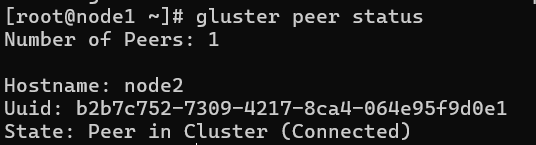
\includegraphics[width=0.8\textwidth]{images/результат создания пула.png}
    \caption{Состояние доверенного пула на node1}
    \label{fig:peer1}
\end{figure}

Расшифровка вывода: \texttt{Number of Peers: 1} --- в пул добавлен
один удалённый узел; \texttt{Hostname} и \texttt{Uuid} --- имя и
уникальный идентификатор пира, которым узлы опознают друг друга
при обмене командами; \texttt{State: Peer in Cluster (Connected)} ---
узел \texttt{node2} является членом кластера и соединение с его
службой \texttt{glusterd} установлено. Доверенный пул из двух
серверов создан.

На рисунке \ref{fig:peer2} представлен вывод состояния пула из консоли node2.
\begin{figure}[h]
    \centering
    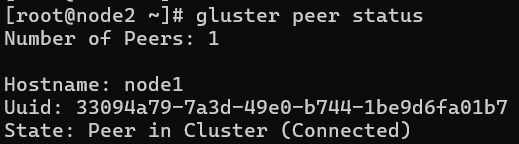
\includegraphics[width=0.8\textwidth]{images/рез создания пула 2.png}
    \caption{Состояние доверенного пула на node2}
    \label{fig:peer2}
\end{figure}

\subsection{Том типа Distributed}

В распределённом (distributed) томе файлы размещаются по брикам
целиком, без создания копий: очередной файл записывается на тот
брик, который выбирается алгоритмом распределения. Объём тома равен
сумме объёмов бриков.

На серверах созданы каталоги-брики (листинг~\ref{lst:dist-brick}).
Флаг \texttt{-p} команды \texttt{mkdir} создаёт всю цепочку
родительских каталогов, если их нет, и не выдаёт ошибку, если
каталог уже существует.

\begin{lstlisting}[caption={Создание бриков (node1, node2)}, label={lst:dist-brick}]
mkdir -p /data/brick1/vdist
\end{lstlisting}

После этого с узла \texttt{node1} создан и запущен том \texttt{vdist}
(листинг~\ref{lst:dist-create}). Разбор команды создания тома:
\texttt{gluster} --- утилита управления GlusterFS;
\texttt{volume create} --- операция создания тома;
\texttt{vdist} --- имя создаваемого тома;
\texttt{node1:/data/brick1/vdist node2:/data/brick1/vdist} --- список
бриков в формате \texttt{узел:каталог}, из которых собирается том;
\texttt{force} --- разрешение использовать корневый раздел под
хранилище (GlusterFS по умолчанию запрещает это и требует явного
подтверждения). Параметр \texttt{replica} не указан, поэтому том
создаётся распределённым. Команда \texttt{volume start} запускает
том. Команда \texttt{volume info} выводит
параметры тома: тип, состояние и список бриков.

\begin{lstlisting}[caption={Создание и запуск тома vdist (node1)}, label={lst:dist-create}]
gluster volume create vdist node1:/data/brick1/vdist node2:/data/brick1/vdist force
gluster volume start vdist
gluster volume info vdist
\end{lstlisting}

Монтирование --- подключение файловой системы к дереву каталогов 
операционной системы: после монтирования
содержимое файловой системы становится доступно через указанный
каталог --- точку монтирования. 
На клиенте \texttt{mgmt} том смонтирован по сети через модуль
FUSE в каталог \texttt{/mnt/vdist} (листинг~\ref{lst:dist-mount}).
Разбор команды: \texttt{mount} --- утилита монтирования;
\texttt{-t glusterfs} --- тип файловой системы;
\texttt{node1:/vdist} --- адрес тома: имя любого сервера пула и имя
тома;
\texttt{/mnt/vdist} --- точка монтирования. Команда \texttt{df -h}
подтверждает монтирование: в колонке Filesystem появляется запись
\texttt{node1:/vdist}.

\begin{lstlisting}[caption={Монтирование тома на клиенте (mgmt)}, label={lst:dist-mount}]
mkdir -p /mnt/vdist
mount -t glusterfs node1:/vdist /mnt/vdist
df -h /mnt/vdist
\end{lstlisting}

Для исследования размещения файлов на бриках с клиента записано
шесть тестовых файлов (листинг~\ref{lst:dist-write}).

\begin{lstlisting}[caption={Запись тестовых файлов (mgmt)}, label={lst:dist-write}]
for i in 1 2 3 4 5 6; do echo "file $i" > /mnt/vdist/file$i.txt; done
ls -l /mnt/vdist
\end{lstlisting}

Содержимое каталогов-бриков на обоих серверах представлено
на рисунках \ref{fig:dist-node1} и \ref{fig:dist-node2}, содержимое
тома на клиенте --- на рисунке \ref{fig:dist-mgmt}.

\begin{figure}[h]
    \centering
    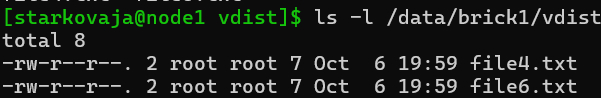
\includegraphics[width=0.8\textwidth]{images/dist_node1.png}
    \caption{Содержимое брика на node1}
    \label{fig:dist-node1}
\end{figure}

\begin{figure}[h]
    \centering
    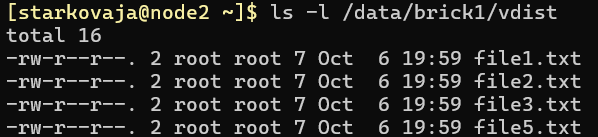
\includegraphics[width=0.8\textwidth]{images/dist_node2.png}
    \caption{Содержимое брика на node2}
    \label{fig:dist-node2}
\end{figure}

\begin{figure}[h!]
    \centering
    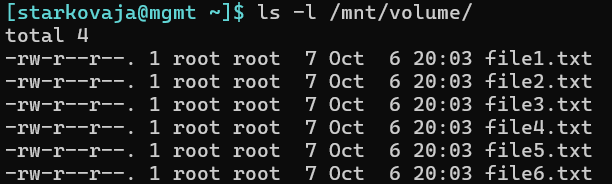
\includegraphics[width=0.8\textwidth]{images/dist_mgmt.png}
    \caption{Содержимое тома на клиенте mgmt}
    \label{fig:dist-mgmt}
\end{figure}

На клиенте (рисунок~\ref{fig:dist-mgmt}) видны все шесть файлов,
однако физически они разделены между серверами: на \texttt{node1}
(рисунок~\ref{fig:dist-node1}) расположены file4.txt и file6.txt,
на \texttt{node2} (рисунок~\ref{fig:dist-node2}) --- file1.txt,
file2.txt, file3.txt и file5.txt. 

\subsection{Том типа Replica}

В реплицированном (replica) томе каждый файл хранится в полной копии
на каждом брике реплик-группы. Объём тома равен объёму одного брика.
Избыточность обеспечивает доступность данных при
отказе любого из серверов. 


Созданы новые брики и том \texttt{vrep} типа replica
(листинг~\ref{lst:rep-create}).

\begin{lstlisting}[caption={Создание бриков (node1, node2)}, label={lst:rep-brick}]
mkdir -p /data/brick1/vrep
\end{lstlisting}

\begin{lstlisting}[caption={Создание и запуск тома vrep (node1)}, label={lst:rep-create}]
gluster volume create vrep replica 2 node1:/data/brick1/vrep node2:/data/brick1/vrep force
gluster volume start vrep
gluster volume info vrep
\end{lstlisting}

В выводе \texttt{volume info} для данного тома указывается
\texttt{Type: Replicate} и \texttt{Number of Bricks: 1 x 2 = 2} ---
одна группа репликации из двух бриков. Том смонтирован на клиенте
в каталог \texttt{/mnt/vrep} (листинг~\ref{lst:rep-mount}), после чего с клиента
записаны шесть тестовых файлов (листинг~\ref{lst:rep-write}).

\begin{lstlisting}[caption={Монтирование тома на клиенте (mgmt)}, label={lst:rep-mount}]
mount -t glusterfs node1:/vrep /mnt/vrep
df -h /mnt/vrep
\end{lstlisting}

\begin{lstlisting}[caption={Запись тестовых файлов (mgmt)}, label={lst:rep-write}]
for i in 1 2 3 4 5 6; do echo "file $i" > /mnt/vrep/file$i.txt; done
ls -l /mnt/vrep
\end{lstlisting}

Содержимое каталогов-бриков на серверах представлено на рисунках
\ref{fig:rep-node1} и \ref{fig:rep-node2}.

\begin{figure}[h]
    \centering
    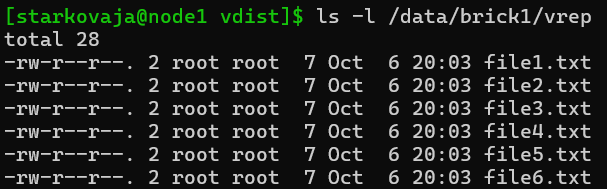
\includegraphics[width=0.8\textwidth]{images/rep_nod1.png}
    \caption{Содержимое брика на node1}
    \label{fig:rep-node1}
\end{figure}

\begin{figure}[h]
    \centering
    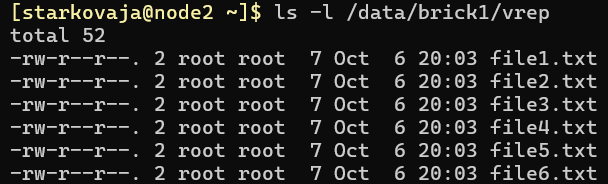
\includegraphics[width=0.8\textwidth]{images/rep_node2.png}
    \caption{Содержимое брика на node2}
    \label{fig:rep-node2}
\end{figure}

\subsection{Том типа Replica с арбитром}

Том типа replica с арбитром содержит две полные копии данных и
один брик-арбитр, хранящий только метаданные --- имена и атрибуты
файлов. Арбитр позволяет кластеру разрешать конфликты при
нарушении связности. В целях демонстрации на двух серверах
брик арбитра размещён на \texttt{node1}.

Созданы каталоги-брики (листинг~\ref{lst:arb-brick}): два брика
с данными --- на обоих серверах, брик арбитра --- на \texttt{node1}.

\begin{lstlisting}[caption={Создание бриков (node1, node2)}, label={lst:arb-brick}]
# node1, node2
mkdir -p /data/brick1/varb

# node1
mkdir -p /data/arb/varb
\end{lstlisting}

Создан и запущен том \texttt{varb} (листинг~\ref{lst:arb-create}).
Параметры \texttt{replica 2 arbiter 1} задают группу репликации
из двух бриков данных и одного брика-арбитра.

\begin{lstlisting}[caption={Создание и запуск тома varb (node1)}, label={lst:arb-create}]
gluster volume create varb replica 2 arbiter 1 \
  node1:/data/brick1/varb node2:/data/brick1/varb node1:/data/arb/varb force
gluster volume start varb
gluster volume info varb
\end{lstlisting}

В выводе \texttt{volume info} для данного тома указывается
\texttt{Type: Replicate} и \texttt{Number of Bricks: 1 x (2 + 1) = 3}
--- одна группа репликации из двух бриков данных и одного брика
арбитра, при этом третий брик помечен как \texttt{(arbiter)}.
Том смонтирован на клиенте (листинг~\ref{lst:arb-mount}),
после чего с клиента записаны три тестовых файла
(листинг~\ref{lst:arb-write}).

\begin{lstlisting}[caption={Монтирование тома на клиенте (mgmt)}, label={lst:arb-mount}]
mkdir -p /mnt/varb
mount -t glusterfs node1:/varb /mnt/varb
df -h /mnt/varb
\end{lstlisting}

\begin{lstlisting}[caption={Запись тестовых файлов (mgmt)}, label={lst:arb-write}]
for i in 1 2 3; do echo "file $i" > /mnt/varb/file$i.txt; done
ls -l /mnt/varb
\end{lstlisting}

Физическое размещение файлов: на бриках данных\\
(\texttt{node1:/data/brick1/varb} и \texttt{node2:/data/brick1/varb})
файлы имеют размер 7 байт (полное содержимое), а на брике-арбитре
(\texttt{node1:/data/arb/varb}) --- те же файлы размером 0 байт.

\subsection{Том типа Dispersed}

Дисперсный (dispersed) том использует избыточное кодирование: 
каждый файл разбивается на фрагменты данных и
блоки чётности, которые распределяются по всем брикам
дисперс-группы. Параметры \texttt{disperse 3 redundancy 1} задают
группу из трёх бриков, из которых один хранит чётность: том
переживает отказ любого одного брика при избыточности 1.5x
(против 2x у реплики). Как и в случае арбитра, в целях
демонстрации на двух серверах третий брик размещён на
\texttt{node1} (параметр \texttt{force}).

Созданы каталоги-брики (листинг~\ref{lst:disp-brick}).

\begin{lstlisting}[caption={Создание бриков (node1, node2)}, label={lst:disp-brick}]
# node1, node2
mkdir -p /data/brick1/vdisp

# node1
mkdir -p /data/disp2/vdisp
\end{lstlisting}

Создан и запущен том \texttt{vdisp} (листинг~\ref{lst:disp-create}).

\begin{lstlisting}[caption={Создание и запуск тома vdisp (node1)}, label={lst:disp-create}]
gluster volume create vdisp disperse 3 redundancy 1 \
  node1:/data/brick1/vdisp node2:/data/brick1/vdisp node1:/data/disp2/vdisp force
gluster volume start vdisp
gluster volume info vdisp
\end{lstlisting}

В выводе \texttt{volume info} указывается:
\\\texttt{Type: Disperse},
\\\texttt{Number of Bricks: 1 x 3 = 3}, 
\\\texttt{Disperse-count: 3},
\\\texttt{Redundancy-count: 1}. 
\\Том смонтирован на клиенте
(листинг~\ref{lst:disp-mount}), после чего с клиента записаны
три тестовых файла (листинг~\ref{lst:disp-write}).

\begin{lstlisting}[caption={Монтирование тома на клиенте (mgmt)}, label={lst:disp-mount}]
mkdir -p /mnt/vdisp
mount -t glusterfs node1:/vdisp /mnt/vdisp
df -h /mnt/vdisp
\end{lstlisting}

\begin{lstlisting}[caption={Запись тестовых файлов (mgmt)}, label={lst:disp-write}]
for i in 1 2 3; do echo "file $i" > /mnt/vdisp/file$i.txt; done
ls -l /mnt/vdisp
\end{lstlisting}

Физическое размещение файлов: на каждом из трёх бриков
находятся фрагменты всех трёх файлов размером 512 байт ---
это размер блока избыточного кодирования. Файл не хранится
целиком ни на одном брике, в отличие от распределённого тома и реплицированного.
При чтении через смонтированный том
клиент видит файлы исходного размера 7 байт --- GlusterFS
автоматически собирает файл из фрагментов.

\subsection{Квоты}

Квота (quota) --- ограничение объёма данных, разрешённого для записи
в том целиком или в отдельном каталоге тома. GlusterFS поддерживает
жёсткий лимит (hard limit), при достижении которого запись
запрещается, и мягкий лимит (soft limit), по умолчанию равный
80\% от жёсткого. Квоты работают на томе \texttt{vrep}.

Том \texttt{vrep} предварительно смонтирован на клиенте
(листинг~\ref{lst:quota-mount}).

\begin{lstlisting}[caption={Монтирование тома vrep на клиенте (mgmt)}, label={lst:quota-mount}]
mount -t glusterfs node1:/vrep /mnt/vrep
df -h /mnt/vrep
\end{lstlisting}

После этого на клиенте создан каталог, на который назначен лимит,
а на узле \texttt{node1} включён механизм квот и установлен лимит
10 МБ на каталог \texttt{/project} (листинг~\ref{lst:quota-set}).

\begin{lstlisting}[caption={Включение квот и установка лимита (mgmt, node1)}, label={lst:quota-set}]
# mgmt
mkdir -p /mnt/vrep/project

# node1
gluster volume quota vrep enable
gluster volume quota vrep limit-usage /project 10MB
gluster volume quota vrep soft-timeout 0
gluster volume quota vrep hard-timeout 0
\end{lstlisting}

Параметры \texttt{soft-timeout} и \texttt{hard-timeout}, установленные
в ноль, отключают задержку применения лимита: по умолчанию учёт
квот обновляется с задержкой в несколько секунд, и быстрая запись
успевает превысить лимит до его проверки.

Для проверки с клиента последовательно записаны два файла: 5 МБ и
8 МБ (листинг~\ref{lst:quota-test}). Первый файл помещается в лимит,
вторая запись обрывается ошибкой \texttt{Disk quota exceeded},
так как суммарный объём превысил бы 10 МБ.

\begin{lstlisting}[caption={Проверка квоты (mgmt)}, label={lst:quota-test}]
dd if=/dev/zero of=/mnt/vrep/project/f1 bs=1M count=5
dd if=/dev/zero of=/mnt/vrep/project/f2 bs=1M count=8
\end{lstlisting}

Результат записи файлов:
первая команда завершилась успешно, вторая оборвалась ошибкой
\texttt{Disk quota exceeded}.


Статистика квот (листинг~\ref{lst:quota-list}) показывает, что каталог
\texttt{/project} занял 10.0 МБ из разрешённых 10.0 МБ, лимит
превышен (\texttt{Hard exceeded? Yes}), доступный объём --- 0 байт.


\begin{lstlisting}[caption={Статистика квот (node1)}, label={lst:quota-list}]
gluster volume quota vrep list
\end{lstlisting}


\subsection{Снимки}

Снимок (snapshot) фиксирует состояние тома на момент создания.
Снимки GlusterFS построены на механизме тонких томов LVM
(thin LVM): снимок не копирует данные, а фиксирует текущие блоки
тонкого тома, поэтому создаётся мгновенно, а изменения после
снимка записываются в новые блоки (copy-on-write). Следствие ---
брики тома должны размещаться на тонких логических томах LVM,
а не в каталоге корневой файловой системы.

На серверы добавлены виртуальные диски объёмом 4 ГБ. На каждом
сервере создан физический том, группа томов \texttt{bricks},
тонкий пул \texttt{pool0} и тонкий том \texttt{snapbrick} объёмом
2 ГБ с файловой системой XFS (листинг~\ref{lst:thin-lvm}). 
Для автоматического монтирования
после перезагрузки в файл \texttt{/etc/fstab} добавлена запись.

\begin{lstlisting}[caption={Развертывание thin LVM (node1, node2)}, label={lst:thin-lvm}]
pvcreate /dev/sdb
vgcreate bricks /dev/sdb
lvcreate --type thin-pool --name pool0 --extents 100%FREE bricks
lvcreate --type thin --name snapbrick --virtualsize 2G --thinpool bricks/pool0
mkfs.xfs /dev/bricks/snapbrick
mkdir -p /data/lvm1
mount /dev/bricks/snapbrick /data/lvm1
echo '/dev/bricks/snapbrick /data/lvm1 xfs defaults 0 0' >> /etc/fstab
\end{lstlisting}

На бриках тонкого тома создан и запущен том \texttt{snapvol},
который смонтирован на клиенте (листинг~\ref{lst:snapvol}).
Параметр \texttt{force} здесь не требуется --- брики размещены
на отдельной файловой системе.

\begin{lstlisting}[caption={Создание тома snapvol и монтирование (node1, node2, mgmt)}, label={lst:snapvol}]
# node1, node2
mkdir -p /data/lvm1/snapvol

# node1
gluster volume create snapvol node1:/data/lvm1/snapvol node2:/data/lvm1/snapvol
gluster volume start snapvol

# mgmt
mkdir -p /mnt/snapvol
mount -t glusterfs node1:/snapvol /mnt/snapvol
\end{lstlisting}

Создан файл \texttt{doc.txt} с содержимым «version 1» --- состояние
«до» (листинг~\ref{lst:snap-before}). С узла \texttt{node1}
выполнено создание снимка \texttt{snap1}; флаг \texttt{no-timestamp}
запрещает добавление даты к имени снимка
(листинг~\ref{lst:snap-create}).

\begin{lstlisting}[caption={Состояние "до" (mgmt)}, label={lst:snap-before}]
echo "version 1" > /mnt/snapvol/doc.txt
cat /mnt/snapvol/doc.txt
\end{lstlisting}

\begin{lstlisting}[caption={Создание снимка (node1)}, label={lst:snap-create}]
gluster snapshot create snap1 snapvol no-timestamp
gluster snapshot list
\end{lstlisting}

После создания снимка файл изменён («version 2») и добавлен файл
\texttt{new.txt} --- состояние «после»
(листинг~\ref{lst:snap-change}).

\begin{lstlisting}[caption={Состояние "после" (mgmt)}, label={lst:snap-change}]
echo "version 2" > /mnt/snapvol/doc.txt
echo "new file" > /mnt/snapvol/new.txt
ls -l /mnt/snapvol
\end{lstlisting}

Для просмотра снимка он активирован на \texttt{node1}, после чего
на клиенте смонтирован по специальному пути
\texttt{node1:/snaps/snap1/snapvol} в каталог \texttt{/mnt/snap1}
(листинг~\ref{lst:snap-activate}). Снимок доступен только
для чтения.

\begin{lstlisting}[caption={Активация и монтирование снимка (node1, mgmt)}, label={lst:snap-activate}]
# node1
gluster snapshot activate snap1

# mgmt
mkdir -p /mnt/snap1
mount -t glusterfs node1:/snaps/snap1/snapvol /mnt/snap1
\end{lstlisting}

Сравнение содержимого живого тома и снимка
(листинг~\ref{lst:snap-compare}): в живом томе \texttt{doc.txt}
содержит «version 2», в снимке --- «version 1»; файл
\texttt{new.txt} в снимке отсутствует. Снимок фиксирует
состояние данных на момент его создания.

\begin{lstlisting}[caption={Сравнение живого тома и снимка (mgmt)}, label={lst:snap-compare}]
cat /mnt/snapvol/doc.txt     # version 2
cat /mnt/snap1/doc.txt       # version 1
ls /mnt/snap1                # no new.txt 
\end{lstlisting}

Для восстановления на клиенте отмонтированы снимок и том, после
чего на \texttt{node1} выполнены остановка тома, откат к снимку
и повторный запуск (листинг~\ref{lst:snap-restore}). Команда
\texttt{snapshot restore} заменяет текущее состояние тома
состоянием снимка: все изменения, выполненные после создания
снимка, утрачиваются.

\begin{lstlisting}[caption={Восстановление тома из снимка (mgmt, node1)}, label={lst:snap-restore}]
# mgmt
umount /mnt/snap1
umount /mnt/snapvol

# node1
gluster volume stop snapvol
gluster snapshot restore snap1
gluster volume start snapvol

# mgmt
mount -t glusterfs node1:/snapvol /mnt/snapvol
\end{lstlisting}

Результат восстановления представлен в
листинге~\ref{lst:snap-verify}: файл \texttt{doc.txt} вернулся
к содержимому «version 1», файл \texttt{new.txt} исчез,
а использованный снимок автоматически удалён --- команда
\texttt{gluster snapshot list} сообщает \texttt{No snapshots
present}.

\begin{lstlisting}[caption={Проверка результата восстановления (mgmt, node1)}, label={lst:snap-verify}]
# mgmt
cat /mnt/snapvol/doc.txt     # version 1
ls /mnt/snapvol              # no new.txt 

# node1
gluster snapshot list        # No snapshots present
\end{lstlisting}

\subsection{Удаление тома}

Удаление тома выполняется в строгом порядке: отмонтирование тома
на клиенте, остановка тома, удаление тома из кластера и очистка
каталогов-бриков на серверах (листинг~\ref{lst:vol-delete}).
Очистка каталогов обязательна: команда \texttt{volume delete}
удаляет только описание тома из конфигурации кластера, а в каталоге
брика остаются служебный каталог \texttt{.glusterfs} и расширенные
атрибуты; повторное использование такого каталога невозможно ---
GlusterFS сообщит, что он \texttt{is already part of a volume}.
Порядок удаления продемонстрирован на томе \texttt{vdist}.

\begin{lstlisting}[caption={Удаление тома vdist (mgmt, node1, node1 и node2)}, label={lst:vol-delete}]
# mgmt
umount /mnt/vdist

# node1
gluster volume stop vdist
gluster volume delete vdist
gluster volume list

# node1, node2
rm -rf /data/brick1/vdist
\end{lstlisting}

После выполнения команд том \texttt{vdist} исчезает из вывода
\texttt{gluster volume list}, каталоги-брики на серверах очищены.